\let\negmedspace\undefined
\let\negthickspace\undefined
\documentclass[journal]{IEEEtran}
\usepackage[a5paper, margin=10mm, onecolumn]{geometry}
%\usepackage{lmodern} % Ensure lmodern is loaded for pdflatex
\usepackage{tfrupee} % Include tfrupee package

\setlength{\headheight}{1cm} % Set the height of the header box
\setlength{\headsep}{0mm}     % Set the distance between the header box and the top of the text

\usepackage{gvv-book}
\usepackage{gvv}
\usepackage{cite}
\usepackage{physics}
\usepackage{amsmath,amssymb,amsfonts,amsthm}
\usepackage{algorithmic}
\usepackage{graphicx}
\usepackage{textcomp}
\usepackage{xcolor}
\usepackage{txfonts}
\usepackage{listings}
\usepackage{enumitem}
\usepackage{mathtools}
\usepackage{gensymb}
\usepackage{comment}
\usepackage[breaklinks=true]{hyperref}
\usepackage{tkz-euclide} 
\usepackage{listings}
% \usepackage{gvv}                                        
\def\inputGnumericTable{}                                 
\usepackage[latin1]{inputenc}                                
\usepackage{color}                                            
\usepackage{array}                                            
\usepackage{longtable}                                       
\usepackage{calc}                                             
\usepackage{multirow}                                         
\usepackage{hhline}                                           
\usepackage{ifthen}                                           
\usepackage{lscape}
\begin{document}

\bibliographystyle{IEEEtran}

\title{2.8.2}
\author{EE25BTECH11023 - Venkata Sai}
% \maketitle
% \newpage
% \bigskip
{\let\newpage\relax\maketitle}

\renewcommand{\thefigure}{\theenumi}
\renewcommand{\thetable}{\theenumi}
\setlength{\intextsep}{10pt} % Space between text and floats


\numberwithin{align}{enumi}
\numberwithin{figure}{enumi}
\renewcommand{\thetable}{\theenumi}

\textbf{Question}:\newline
$\vec{A}\brak{6,1},\vec{B}\brak{8, 2}$ and $\vec{C}\brak{9, 4}$ are three vertices of a parallelogram $ABCD$. If E is the
midpoint of DC find the area of $\triangle$ADE. 
\\

\textbf{Solution:}

Given:
\begin{align}
\vec{A}=\myvec{6\\1},\ 
\vec{B}=\myvec{8\\2},\ 
\vec{C}=\myvec{9\\4}.
\end{align}

As $ABCD$ is a parallelogram with $AB$ $\parallel$ $CD$;
\begin{align}
    \vec{B}&-\vec{A}=\vec{C}-\vec{D} \\
    \vec{D}&=\vec{C}+\vec{A}-\vec{B} \\
    \vec{D}&=\myvec{9\\4}+\myvec{6\\1}-\myvec{8\\2} \\
    \vec{D}&=\myvec{7\\3}
\end{align}

Finding Area Of $\triangle{ADE}$:
\begin{align}
\vec{E}=\frac{\vec{D}+\vec{C}}2 =\frac{\myvec{7\\3}+\myvec{9\\4}}2=\myvec{8\\\frac{7}2} 
\end{align}
\begin{align}
\vec{D}-\vec{A}=\myvec{7\\3}-\myvec{6\\1}=\myvec{1\\2},\vec{E}-\vec{A}=\myvec{8\\\frac72}-\myvec{6\\1}=\myvec{2\\\frac52} 
\end{align}
\begin{align}
\text{Area\brak{\triangle ADE}}&=\frac12\norm{\brak{\vec{D}-\vec{A}}\times\brak{\vec{E}-\vec{A}}}. \\
& =\frac12\norm{\myvec{1\\2}\times \myvec{2\\\frac52}} = \frac{1}{2}\mdet{1 & 2 \\ 2 & \frac{5}{2}}=\frac{3}{4} 
\end{align}

\begin{figure}[h!]
   \centering
   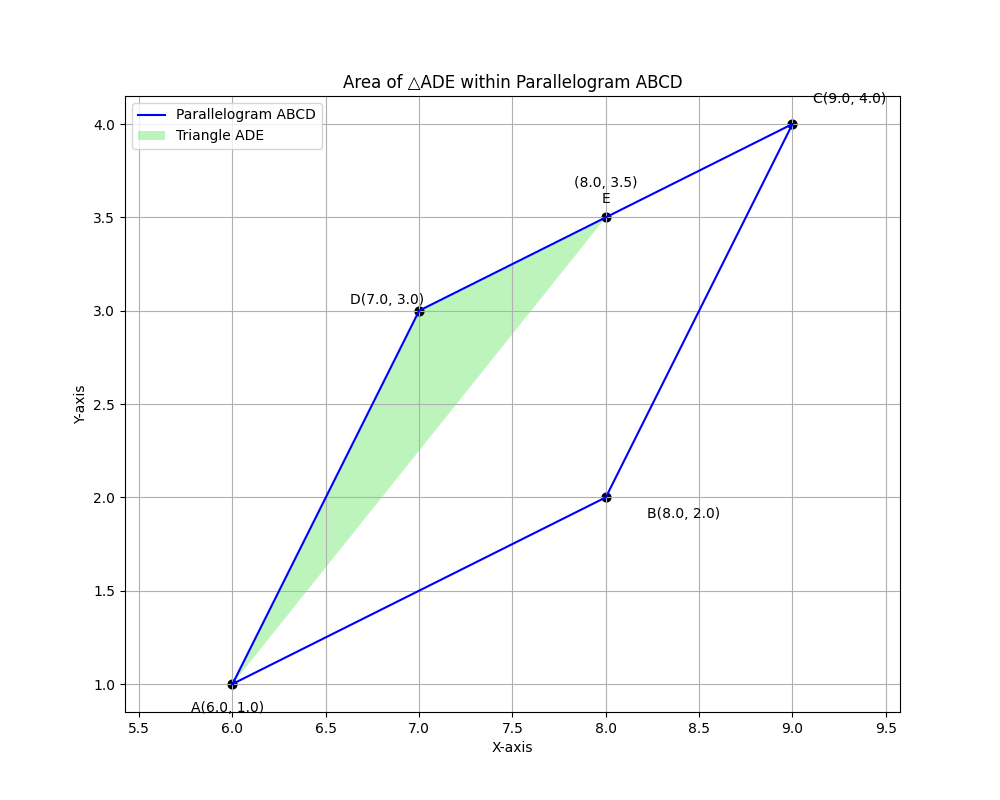
\includegraphics[width=0.7\columnwidth]{figs/fig1.png}
   \caption{Area}
   \label{stemplot}
\end{figure}
\end{document}  
